\documentclass[../SimBALink.tex]{subfiles}
\begin{document}

\subsection{Tires}
\subsection{Inputs and outputs}
	\subsubsection{Inputs}
	\begin{tabular}{ l | l | l  }
		Input					&	Symbol		&	Unit		\\	\hline
		Brake Force				& 	$F_b$ 		&	N \\
		Gear Torque				&	$\tau_g$	&	Nm \\
		Wheel Forces[3]			&	$F_w$		&	N[3] \\
		Vehicle Velocity		&	$v$			&	m/s \\
		Lead Angle				&	$\theta_l$	&	rad \\
	\end{tabular}
	
	\subsubsection{Outputs}
	\begin{tabular}{ l | l | l  }
		Output					&	Symbol			&	Unit		\\	\hline
		Tire Torque				&	$\tau_t$		&	Nm \\
		Acceleration Force		&	$F_a$			&	N \\
		Acceleration Torque		&	$\tau_a$		&	Nm \\
		Tire Road Torque		&	$\tau_r$		&	Nm \\
		Wheel Slip				&	$\kappa$ 		&	ratio \\ 			
		Max Force 				&	$F_{max}$		&	N \\
	\end{tabular}

\subsubsection{Background, rationale, modeling strategy} The tire is modeled in three parts, rolling resistance, Load and Torque, and Traction Limiting. Force directions are defined as longitudinal(long), lateral(lat), and normal(n). Longitudinal is along the direction of the motorcycle (when moving straight). Lateral is orthogonal to Longitudinal axis. Normal 3-D orthogonal to lateral and longitudinal, in general the axis to the road on no incline.

The tire models slip which in turn is used to calculate the force the tire exerts on to the motorcycle. Wheel slip occurs when because the the tire does not exert a force on to the vehicle until there is some wheel slip, thus causing the tire to spin up causing wheel slip.

\begin{gather}
\notag \textbf{Rolling Resistance} \\
Frr = 
\left\{
  \begin{array}{lr}
    (0.0085 + \frac{0.18}{p_t} + \frac{1.59*10^{-6}}{p_t}v_{kph}^2)F_{w,n} & : v_{kph} \le 165 (km/h)\\
    (\frac{0.18}{p_t} + \frac{2.91*10^{-6}}{p_t}v_{kph}^2)F_{w,n} & : v_{kph} > 165 (km/h)
  \end{array}
\right. \\
\notag \textbf{Wheel Slip} \\
\kappa = -\frac{v - \omega_t r_t(\theta_l)}{v} \\
\mu_{t,gnd} =  D_{\kappa}\sin(C_{\kappa} \arctan[B_{\kappa}\kappa - E_{\kappa}(B_{\kappa}\kappa - \arctan B_{\kappa}\kappa)])  \\
\notag \textbf{Load and Torque} \\
\tau_r = F_{w,long}r_t(\theta_l) + F_br_b + F_{rr}r_t(\theta_l) \\
\notag \textbf{Traction Limiting} \\
F_a = \mu_{t,gnd} F_{w,n} - F_{w,long} \\
\notag \textbf{Torque on Chain/Gear} \\
\tau_a = F_ar_t(\theta_l) \\
\tau_t = \tau_a + \tau_r
\end{gather}

The tire coefficient ($\mu_{t,gnd}$) is modeled using the "Magic Formula" as shown below. Where $D_{\kappa}$ is the maximum tire coefficient of the tire. 

 \begin{figure}[H]
  \centering
  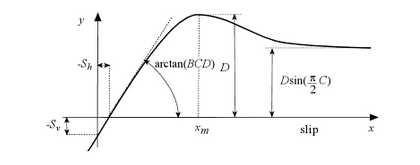
\includegraphics[scale=1]{magic_formula}
  \caption{Magic Formula }
\end{figure}

\subsubsection{Variables}
	\begin{tabular}{ l | l | l  }
		Var					&	Symbol		&	Unit		\\	\hline
		Rolling Constant	&	$K_t$		& 	n/a \\
		Tire coefficient 	& $\mu_{t,gnd}$ &	n/a \\
		Force 				&	$F$	&	N \\
	\end{tabular}
\subsubsection{Parameters}
	\begin{tabular}{ l | l | l  }
		Param.					&	Symbol		&	Unit		\\	\hline
		Tire Pressure		&	$p_t$		&	 $bar$ \\
		Brake Caliper Radius &	$r_b$		&	m \\		
		\textbf{Magic Formula}\\		&	$A_{\kappa},B_{\kappa},C_{\kappa},D_{\kappa}$		&	 n/a \\
	\end{tabular}
	
\subsubsection{Function}
$r_t(\theta_l)$ \\
	\begin{tabular}{ l | l | l | l }
		Type				& Description		&	Symbol		&	Unit		\\	\hline
		Input 				& Lean Angle		&	$\theta_l$  & 	rad		\\
		Output 				& Tire Radius		&	n/a			&	m
	\end{tabular} \\

\subsubsection{Assumptions}
\begin{itemize}
  \item Maximum acceleration force should also depend on lateral forces on the vehicle. However this is not modeled because it requires modeling of high-side and low-side dynamics. The Rider model should control for a safe operating area of the motorcycle to compensate for this assumption. 
  \item No tire deformation
  \item No tire temperature dynamics
  \item No change in rolling resistance with lean angle 
\end{itemize}

\section{Validation}

The tire model was swept through different slip speeds to validate correct shapes. All validation looks correct but multiple parts need to be connected to check for proper dynamics. 

\begin{figure}[H]
\center
 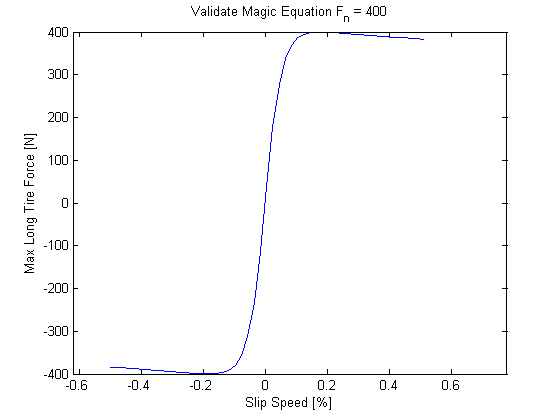
\includegraphics[scale=1]{tire_val_magic}
  \caption{Tire Validation}
\end{figure}

\end{document}